\section{Implementation}
\label{sec:implementation}

\subsection{System Design}

- add system block diagram
- 

\subsection{Camera Sensor Proof of Concept}
- how many photodiodes can we use? how small can we get them to be? area of photodiodes ==> how much photocurrent. therefore, setup an experiment with a RPI HQ camera sensor and see view the resulting speckle pattern. 
translate the house and watch the speckle pattern translate too. use red laser as the wavelength doesnt for easy experimentation.

video of the speckle pattern motion

\subsection{Hardware Implementation}

- photodiodes are typically amplified by TIA. there are other possibilities, like the current integrator (DDC118)
- this application aims to capture high freq up to 1khz, so we have the following opamp requirements:
-> at least 2 opamps in 1 package
-> price around 5usd per chip
-> JFET inputs / low input capacitance
-> operable on a single supply

- thus the choice of amplifier --> OPA2380 with 90 MHZ, 2 opamps per chip, 5 usd

\subsection{Signal Processing}
- rpi with two types of ADC were used
- first ADC was unable to sample at high enough frequencies. it used a MUX but the channel switching was controlled via SPI. therefore the switching delay was hard to control and introduced a high amount of noise. Github issues online also found this issue to be limiting.
- a second ADC was tried, that has a higher sample rate and advertised synchronous sample readout capability. this ADC is a raspberry pi hat and uses the Pis 5V supply as its analog reference, which is very noisy, with peak to peak noise in the millivolt range. To mitigate this issue, a bench supply powered the ADC externally.
- ADC raw data was recorded and observed in realtime or post processed. Realtime observations were done while watching the speckle camera and the IR camera simultaneously.

dont forget to mention how speckle size
\cite{specklesize}


\begin{figure}[t]
  \centering
  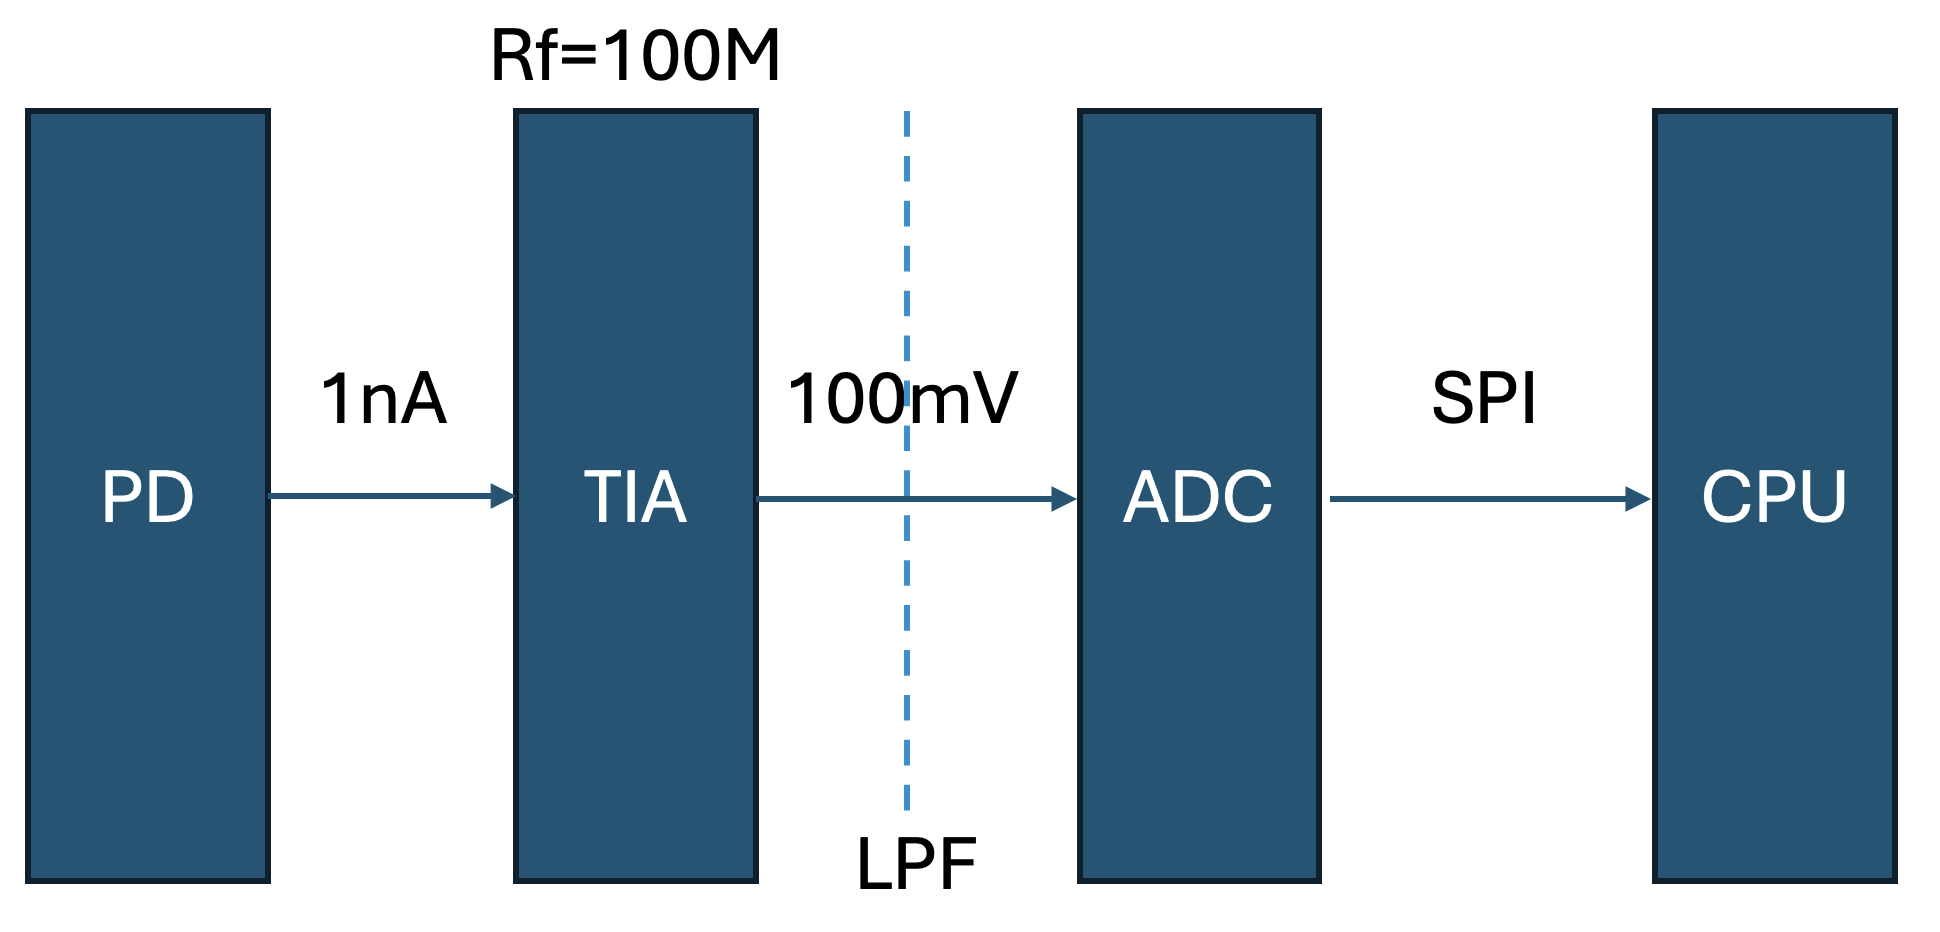
\includegraphics[width=\widthnarrow]{figures/block_diagram.png}
  \caption{Block diagram).}
  \label{fig:something}
\end{figure}



